Stoichiometry is one of the most important skills you need in chemistry, because chemistry is the study of reactions and...well...stoichiometry is the math of reactions. 

\subsection{Introduction}
Let us begin by talking about the story of the Jellybean Shop. Long ago, in the 1970s, candy used to be cheap. Kids used to be able to go into stores with a nickel and come out with a bag full of candy. However, for the shopkeeper, this was no fun business. Kids often asked for 50, 100, even 1000 jellybeans...and the shopkeeper had to count the jelly beans one by one so the kids wouldn't feel like they were getting cheated out. 

One day, the shopkeeper decided that he had to change his ways. He could no longer just count jellybeans one by one---he had to find a faster way. So in his shop, he started weighing individual jellybeans, and he created the following data table.
\begin{center}
\begin{tabular}{|c|c|}
    \hline
     Bean 1 & 0.95 g \\
     Bean 2 & 1.00 g \\
     Bean 3 & 0.98 g \\
     Bean 4 & 0.99 g \\
     Bean 5 & 1.02 g \\
     Bean 6 & 1.01 g \\
     Bean 7 & 0.99 g \\
     Bean 8 & 1.00 g \\
     Bean 9 & 1.03 g \\
     Bean 10 & 1.00 g \\
     \hline
\end{tabular} 
\end{center}
Wow! It turns out that the jellybeans all had a similar mass. The 10 jellybeans he weighed averaged to a mass of 1.003 g/jellybean. Ever since this discovery, the shopkeeper's life has been a lot easier. No longer does he have to labor over counting thousands of jellybeans everyday...one by one. Now, he knows that all he has to do is weigh the mass of jellybeans to determine how many there are. For example, if someone asks for 4729 jellybeans, all he has to do is weigh out:
$$4729 \text{ jellybeans} \times \frac{1.003 \text{ g}}{1 \text{ jellybean}} = \boxed{4743.187 \text{ grams}},$$
or about 4.7 kg. 

At this point, you might be wondering. How does jellybeans have to do with stoichiometry...or even chemistry? Well let me give you a new problem. Suppose I wanted you to figure out how many molecules of oxygen you had in the air, or how many gold atoms were in a bar of gold. Would you grab a super microscope and count all of the atoms and molecules? I hope not.

\subsection{Atomic Mass}
Here we introduce the concept of atomic mass. Just like jellybeans, chemists have so nicely weighed out the masses of atoms and found their average. So the \textbf{atomic mass} of an element is the average mass of an atom. Basically, if you were to measure the masses of a lot of atoms (like a million), their average mass would be the atomic mass. There are complicated reasons why atomic masses aren't perfect (it has to do with isotopes), but we can save that discussion for another day. 

Now let's look at a part of the periodic table to familiarize ourselves with the atomic mass:
\begin{center}
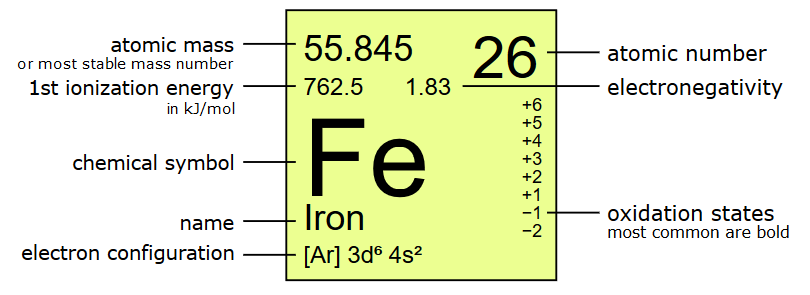
\includegraphics[width=4in]{feLabel}
\end{center}
As you can see, the atomic mass of Fe, or iron, is about 55.85. But what are the units? Grams? No way, one atom of iron is definitely not that heavy. On the periodic table, the units for this mass is 55.85 grams/mole, where the mole is $6.022 \times 10^{23}$ atoms. The \textbf{mole} is defined as the number of carbon atoms in exactly 12 grams of pure carbon-12. For our purposes, the mole is just a big number that helps us make calculations on a reasonable scale. To reinforce what we just learned about jellybeans and atomic mass, let's do a simple problem. 

\begin{problem}
I am told I have a bar of pure gold that has a mass of 4 grams. How many gold atoms are in this bar? 
\end{problem}
\begin{solution}
We begin by identifying the atomic mass of gold, or Au, and find that it is: 196.97 grams/mole. \par
Then, we just divide 4 grams by this atomic mass to figure out the number of moles of gold:
$$4 \text{ g} \times \frac{1 \text{ mol}}{196.97\text{ grams}} = 0.0203 \text{ mole}.$$
And since we know that 1 mole = $6.022 \times 10^{23}$ atoms, 
$$0.0203 \text{ mol} \times \frac{6.022 \times 10^{23} \text{ atoms}}{1 \text{ mole}} = \boxed{1.22 \times 10^{22} \text{ gold atoms}}.$$
That a lot of atoms! This really shows you how small atoms are.
\end{solution}
\begin{problem}
My lab adviser wants me to calculate the number of oxygen atoms in a container that holds 0.800 kg of pure oxygen.
\end{problem}
\begin{problem}
My friend claims that he can life up $1.12\times10^{27}$ atoms of pure silver. Should I believe him?
\end{problem}
\begin{problem}
What is the mass of 1.73 moles of carbon?
\end{problem}

\subsection{Molar Mass}
Ok, so molar mass isn't actually that much different from atomic mass. In fact, if you literally took the definition of atomic mass and replaced ``atom'' with ``molecule'', you'd have the new definition. So here is the definition of \textbf{molar mass}:\textit{the mass of one mole of a compound, also known as molecular mass}. Let's do some problems:

\begin{problem}
Glucose, or \ce{C_6H_{12}O_6} is a very important biological molecule. Calculate its molar mass.
\end{problem}
\begin{problem}
Magnesium Sulfate (\ce{MgSO_4}), also known as Epsom salts, is often used in baths to help sooth sore muscles. If I dump 1 kg of it into my bat, how many moles of \ce{MgSO_4} am I dumping in?
\end{problem}
\begin{problem}
Calculate the percentage masses of each atom in glucose (\ce{C_6H_{12}O_6}).
\end{problem}
\begin{problem}
We now introduce the problem of determining the molecular formula of a compound given its percent compositions. For example, given that a compound has the following:
$$71.65\% \ce{ Cl} \quad 24.27 \% \ce{ C} \quad 4.07 \% \ce{ H},$$
and has a molar mass of 98.96 g/mol, find the empirical and molecular formulas.
\end{problem}
\begin{solution}
We first want to convert the percentage of the elements into masses, and then moles. We find this to be 71.65 g of chlorine, 24.27 g of carbon, and 4.07 g of hydrogen. Now we can calculate the \textit{mole ratio}, by figuring out the proportionate moles of these atoms:
\begin{center}
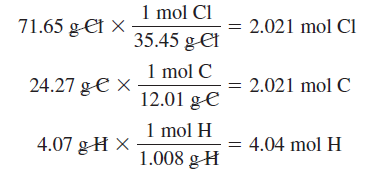
\includegraphics[width=2.5in]{chemEq}
\end{center}
Now we figure out the \textbf{empirical formula}, which is the ratio of atoms in their most simplified form, which means the greatest common factor of the atom ratios is 1. We can do this by dividing our mole ratios by the lowest number, so no we have 
\begin{center}
\begin{tabular}{c|c}
    
    Cl & 1 \\
    C & 1 \\
    H & 2 \\
    
\end{tabular}
\end{center}
So we see that our empirical formula is \ce{ClCH2}. To figure out the molecular formula, we just need to figure out how many molar masses of this empirical formula go into the molecular mass. This is easy because:
$$\frac{\text{Molar mass}}{\text{Empirical formula mass}} = \frac{98.96 \text{ g/mol}}{49.48 \text{ g/mol}} = 2$$
So our final molecular formula is $\boxed{\ce{Cl2C2H4}}$.
\end{solution}
\begin{problem}
A white powder is found to have 43.64 \% phosphorus and 56.36 \% oxygen by mass. If the compound has a molar mass of 283.66 g/mol, what are the empirical and molecular masses of this compound?
\end{problem}
\begin{problem}
Caffeine, a stimulant found in coffee, tea, and chocolate, contains 49.48 \% carbon, 5.15 \% hydrogen, 28.87 \% nitrogen, and 16.49 \% oxygen by mass and has a molar mss of 194.2 g/mol. Determine the molecular formula of caffeine.
\end{problem}
\subsection{Chemical Equations}
Now comes the crux of the power of stoiciometry, chemical equations. Let us start with a simple reaction:
$$\ce{CH4 + 2O2 -> CO2 + 2H2O}$$
On the left hand of the $\rightarrow$, we have the \textbf{reactants}, and on the right side, the \textbf{products}. What this equation tells us is that this reaction takes in the reactants and through a chemical process, makes products. Notice that this equation is \textit{balanced}, that is, the number of atoms on each side are equal. For example, in this one both sides have 1 C, 4 H, and 4 O. \par
Although reactions are a primary part of chemistry, I won't be able to go over all of them in this lecture. I will take liberty and instead talk about doing the equation problems rather than talking about the theory and background of the reactions. This way, you'll be able to do more problems (theory is good but this is an introductory class after all). If you want to learn about reactions, there are plenty of good textbooks out there that can help you. \par
\subsubsection{Balancing Equations}
The first thing we need to do about equations is learn how to balance them. Even though an unbalanced equation tells us what reaction is occurring, if an equation is not balanced, we will not be able to do math with it. \par
As I mentioned earlier, a balanced equation has the same numbers of each atom on each side of the equation. Although there is a systematic way to balance equations, it requires linear algebra (which I imagine would be well beyond what most of you guys have learned so far). Using the trial and error method is pretty strong and fast (much faster than the matrix method) anyway, so let's learn that. \par
Let us start with an equation:
$$\ce{C2H5OH + O2 -> CO2 + H2O}$$
Just FYI, this is an equation representing the reaction between ethanol and oxygen, which produces carbon dioxide and water. The first thing we notice about this equation is that it is clearly not balanced; there are 2 carbons on one side, and there is only one on the other. In order to fix this, we take the following steps:
\begin{enumerate}
    \item Start with the most ``complicated'' (containing the most different types of elements) compound, because this will affect more other compounds in the reaction.
    \begin{enumerate}
        \item In our case, we see that ethanol (\ce{C2H5OH}) is clearly our most complicated molecule.
    \end{enumerate}
    \item Adjust the other molecules based off of this complicated one
        \begin{enumerate}
            \item So now we add a \ce{CO2} to the right side to make $$\ce{C2H5OH + O2 -> 2CO2 + H2O}$$
            \item balance out the hydrogens...
            $$\ce{C2H5OH + O2 -> 2CO2 + 3H2O}$$
        \end{enumerate}
    \item Leave the most ``independent'' molecules at the end. 
        \begin{enumerate}
            \item \ce{O2} is clearly the most independent molecule because it only effects oxygen and no other elements. You want to leave these at the end because they can easily adjust without affecting any work you've done earlier.
            $$\ce{C2H5OH + 3O2 -> 2CO2 + 3H2O}$$
        \end{enumerate}
    \item Check.
        \begin{enumerate}
            \item I know you guys never check your work when you're done because you think: \textit{if I already have the right answer why do I have to check it?} Well the harsh reality is that you don't always have the right answer and that is why checking is important.
            \begin{center}
                \begin{tabular}{c|c}
                    Left & Right \\
                    \hline
                     2 C & 2 C\\
                     6 H & 6 H\\
                     1+6 O & 4+3 O \\
                \end{tabular}
            \end{center}
        \end{enumerate}
    \end{enumerate}
    And if you follow these steps, you should be able to balance any equation. Although the steps don't seem very ``solid'', because it isn't some type of mold you can just use for everything, they still provide a good overall idea and strategy for how to balance equations.
    \subsubsection{Problems}
    \begin{problem}
    When solid ammonium dichromate, \ce{(NH4)2Cr2O7}, a vivid orange compound, is ignited, a spectacular reaction occurs. Balance the equation for the reaction: $$\ce{(NH4)2Cr2O7 -> Cr2O3 + N2 + H2O}$$
    \end{problem}
    \begin{problem}
    Ammonia gas reacts with oxygen gas to form gaseous nitric oxide and water vapor. This reaction is the first step in the commercial production of nitric acid by the Ostwald process. Balance the equation for this reaction:
    $$\ce{NH3 + O2 -> NO + H2O}$$
    \end{problem}
    \subsubsection{Equation Calculations}
    Now we move on to the final and probably most important part of stoichometry, where we answer this question:
    $$\text{\textit{``What mass of oxygen will react with 96.1 grams of propane?''}}$$
    We look at this reaction first:
    $$\ce{C3H8 + O2 -> CO2 + H2O}$$
    At first, we look at this and we think, easy! 96.1 g of propane is just:
    $$96.1 g \times \frac{1 \text{ mol propane}}{44.1 \text{ g propane}} =  2.18 \text{ mol propane}$$
    And since there is one mole of oxygen for each propane, we just need 2.18 mol of oxygen, or just:
    $$2.18 \text{ mol oxygen} \times \frac{32 \text{ g oxygen}}{1 \text{ mol oxygen}} = 69.8 \text{ g oxygen}.$$
    But this is wrong, remember what I said about balancing equations? You have to do that first. Then you can perform your math. \par
    So if we first balance the equation:
    $$\ce{C3H8 + 5O2 -> 3CO2 + 4H2O}$$
    Then we can do our calculation, which will be:
    $$96.1 \text{ g propane} \times \frac{1 \text{ mol propane}}{44.1 \text{ g propane}} \times \frac{1 \text{ mol oxygen}}{1 \text{ mol propane}} \times \frac{32 \text{ g oxygen}}{1 \text{ mol oxygen}} = \boxed{349 \text{ g oxygen}}$$
    Notice that our previous answer was off by a lot (a factor of five). \par
    An overview of how to do chemical reaction problems:
    \begin{enumerate}
        \item Balance the equation for the reaction (MOST IMPORTANT STEP)
        \item Convert the known mass of the reactant or product to moles of that substance (this is important so you can compare apples to apples. Knowing that you have 3 grams of nitrogen tells you nothing about how many grams of ammonia you expect to produce if you don't know the mole ratios)
        \item Use the balanced equation to set up the appropriate mole ratios
        \item Use the appropriate mole ratios to calculate the number of moles of the desired reactant or product
        \item Convert from moles back to grams if required by the problem
    \end{enumerate}
    \subsubsection{Problems}
    \begin{problem}
    Lithium hydroxide is used in space vehicles to remove exhaled carbon dioxide in the living environment through the following reaction
    $$\ce{LiOH + CO2 -> Li2CO3 + H2O}$$
    What mass of carbon dioxide can be absorbed by 1.00 kg of lithium hydroxide?
    \end{problem}
    \begin{problem}
    Baking soda is often used as an antacid. It neutralizes excess hydrochloric acid secreted by the stomach:
    $$\ce{NaHCO3 + HCl -> NaCl + H2O + CO2}.$$
    Milk of magnesia, which is an aqueous suspension of magnesium hydroxide, is also used as an antacid:
    $$\ce{Mg(OH)2 + 2HCl -> 2H2O + MgCl2}$$
    \end{problem}
    \begin{problem}
    Nitrogen gas can be prepared by passing gaseous ammonia over solid copper(II) oxide at high temperatures. The other products of the reaction are solid copper and water vapor. If a sample containing 18.1 g of \ce{NH3} is reacted with 90.4 g of \ce{CuO}, which is the limiting reactant? How many grams of \ce{N2} will be formed? (This is known as the \textbf{limiting reactant} problem)
    \end{problem} 
    \begin{problem}
    Bacterial digestion is an economical method of sewage treatment. The reaction
    $$\ce{5CO2 + 55NH4+ + 76O2 -> C5H7O2N + 54NO2- + 52H2O + 109H+}$$
    is an intermediate step in the conversion of the nitrogen in organic compounds into nitrate ions. What mass of bacterial tissue is produced in a treatment plant for every $1.0 \times 10^4$ kg of wastewater containing 3.0 \% \ce{NH4+} ions by mass? Assume that 95 \% of the ammonium ions are consumed by the bacteria.
    \end{problem} 